\chapter{Results}
\label{sec:results}
% Give the outcomes for each research question in the form of a table or graphic (with caption).
%Write about your results here. Good captions to tables and/or figures are key.

% Sometimes,  especially  if  you  have  quite  different experiments or research  questions,  it makes sense to interleave the experimental setup and the results sections, so the reader does not get lost. It is then helpful to structure clearly in (sub)subsections.

%\section{Table and Figures}
%        \begin{table}[h] % h for Here, t for Top, b for Bottom
%                \centering
%                \caption{By convention, Table caption goes on top.}
%                \begin{tabular}{lcr}
%                        \textbf{Left} & \textbf{center} & \textbf{right} \\
%                        \hline
%                        111 & 222 & 333 \\
%                        444 & 555 & 666
%                \end{tabular}
%        \end{table}

%        \begin{figure}[h]
%                \centering
%                \includegraphics[width=0.5\linewidth]{example-image}
%                \caption[Example figure]{Example figure. Notice that the caption goes below and that there is a way to have a shorter caption for the list of Figures.}
%        \end{figure}

%        \begin{figure*}[b]
%                \centering
%                \includegraphics[width=0.8\linewidth, height=.2\textheight]{example-image}
%                \caption{Example figure spanning the two columns.}
%        \end{figure*}


This chapter presents results for the five research questions introduced before. Section~\ref{sec:rq1} establishes that synthesis is feasible for most APIs. Section~\ref{sec:rq2} shows that synthesized
servers enable effective agent task completion and compares against
human-authored references. Section~\ref{sec:rq3} characterises how
synthesizers rely on parametric knowledge and when this affects downstream
performance. Section~\ref{sec:rq4} examines the effect of documentation
availability. Section~\ref{sec:rq5} quantifies the relationship between
synthesis quality and agent pass rate.
Section~\ref{sec:model_comparison} extends the analysis to seven synthesis models
on a common three-API evaluation set.

% ------------------------------------------------------------
\section{RQ1: Synthesis Feasibility}
\label{sec:rq1}
% ------------------------------------------------------------

\textbf{Can LLMs synthesize functional API tool servers from documentation alone?}

Figure~\ref{fig:heatmap} shows PASS and SYNTH across all 14 APIs and three
synthesis conditions. Twelve of 14 APIs achieve SYNTH $\geq 75\%$ in the
docs condition, with a median of approximately 84\%. Only Jira (56\%) and
eBay Sell (43\%) fall consistently below that threshold, indicating that
synthesis is feasible for the large majority of APIs tested.

The dominant failure mode is \emph{coverage gap}: the server starts and
runs correctly, but the synthesizer omits the specific endpoints required
by certain benchmark tasks. This is most pronounced for large APIs with many endpoints (eBay Sell, Jira), consistent with the negative trend between
endpoint count and SYNTH visible in Figure~\ref{fig:complexity}. Structural
failure --- servers that crash or omit the required \texttt{server.py}
entrypoint entirely --- is rare with GPT-5.2 (the primary synthesis model)
and occurs mainly with weaker or smaller models.

SYNTH is also notably stable across conditions for most APIs: Confluence
holds at 95\% across all three conditions and Mastodon at 93--100\%,
indicating that synthesis quality is primarily determined by API structure
rather than what context is provided. The exceptions --- eBay Commerce drops from SYNTH=100\% (docs) to 54\% (mutated) --- arise where parameter
mutations reduce tool coverage directly.

Grounding analysis shows that synthesizers consistently anchor tools to
real documentation sources: citation validity is 86--100\% across datasets
(every \texttt{grounding.json} entry points to an existing file with a
syntactically plausible endpoint string), and grounding coverage is complete (every synthesized tool has a corresponding entry). This rules out the possibility that high SYNTH scores are driven entirely by tools whose implementations are unmoored from any documentation --- though it does not verify that each tool correctly implements what its cited document describes. Even in the no-docs condition, SYNTH remains high for well-known APIs (GitHub nodocs SYNTH=87\%), suggesting that parametric knowledge can partially substitute for documentation at the synthesis stage --- a finding developed further in Section~\ref{sec:rq3}.

\begin{table}[htbp]
  \centering
  \caption{Agent pass rate (PASS, \%) per API and synthesis condition.
    Rows sorted by mean PASS descending. \textbf{Bold} marks the highest
    value in each row. \colorbox{red!12}{Red} cells indicate PASS $< 50\%$.
    PASS = agent pass rate on scoreable tasks. Heatmap (Fig.~\ref{fig:heatmap}) shows SYNTH alongside PASS.}
  \label{tab:pass_results}
  \setlength{\tabcolsep}{5pt}
  \small
  \begin{tabular}{lrrr}
    \toprule
    \textbf{Dataset} & \textbf{With docs} & \textbf{No docs} & \textbf{Mutated params} \\
    \midrule
    Mastodon         & \textbf{100} & \textbf{100} & \textbf{100} \\
    OpenWeatherMap   & \textbf{100} &           86 & \textbf{100} \\
    Spoonacular      & \textbf{100} &           90 &           78 \\
    Notion           &           78 & \textbf{100} & \textbf{100} \\
    Confluence       &           92 &           93 & \textbf{91}  \\
    Alphavantage     &           86 &           90 & \textbf{88}  \\
    eBay Commerce    & \textbf{100} &           89 &           55 \\
    Shopify          &           87 & \textbf{92}  &           62 \\
    GitHub           &           62 & \textbf{83}  &           76 \\
    eBay Buy         &           73 &           67 & \textbf{80}  \\
    Zulip            & \textbf{80}  &           60 &           62 \\
    Stripe           & \textbf{72}  &           62 &           57 \\
    eBay Sell        &           38 & \textbf{50}  & \cellcolor{red!12}43 \\
    Jira             & \textbf{50}  & \cellcolor{red!12}25 & \textbf{50} \\
    \midrule
    \textit{Median}  &           80 &           86 &           77 \\
    \bottomrule
  \end{tabular}
\end{table}

\begin{figure}[htbp]
  \centering
  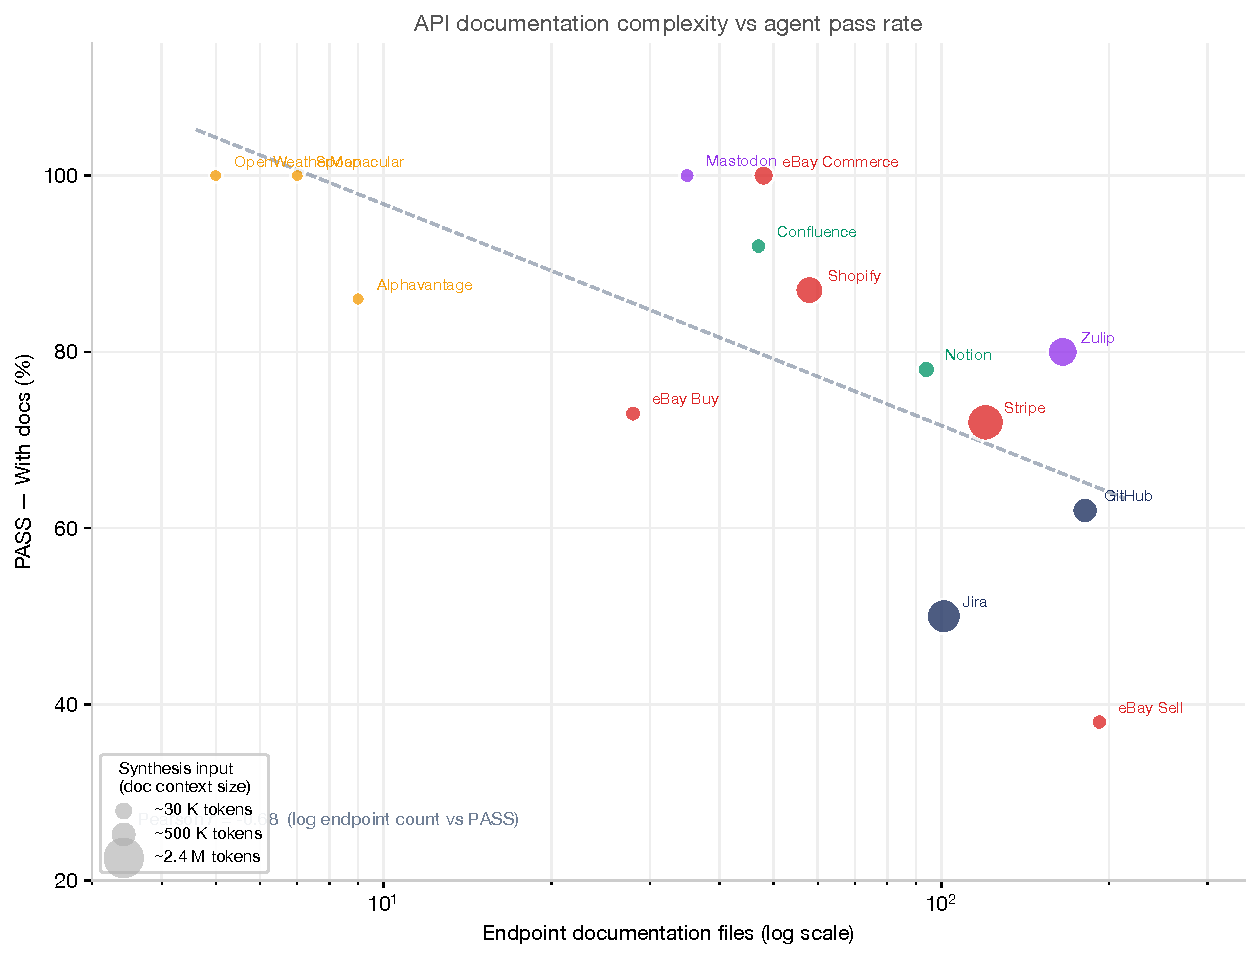
\includegraphics[width=\linewidth]{media/fig8_api_complexity.pdf}
  \caption{Endpoint documentation file count (log scale) vs.\ agent pass rate
    (docs condition). Marker size encodes synthesis input token volume.
    Dashed line is a log-linear fit. Larger APIs with denser documentation
    systematically yield lower PASS, driven by coverage gaps rather than
    server errors.}
  \label{fig:complexity}
\end{figure}

\begin{figure}[htbp]
  \centering
  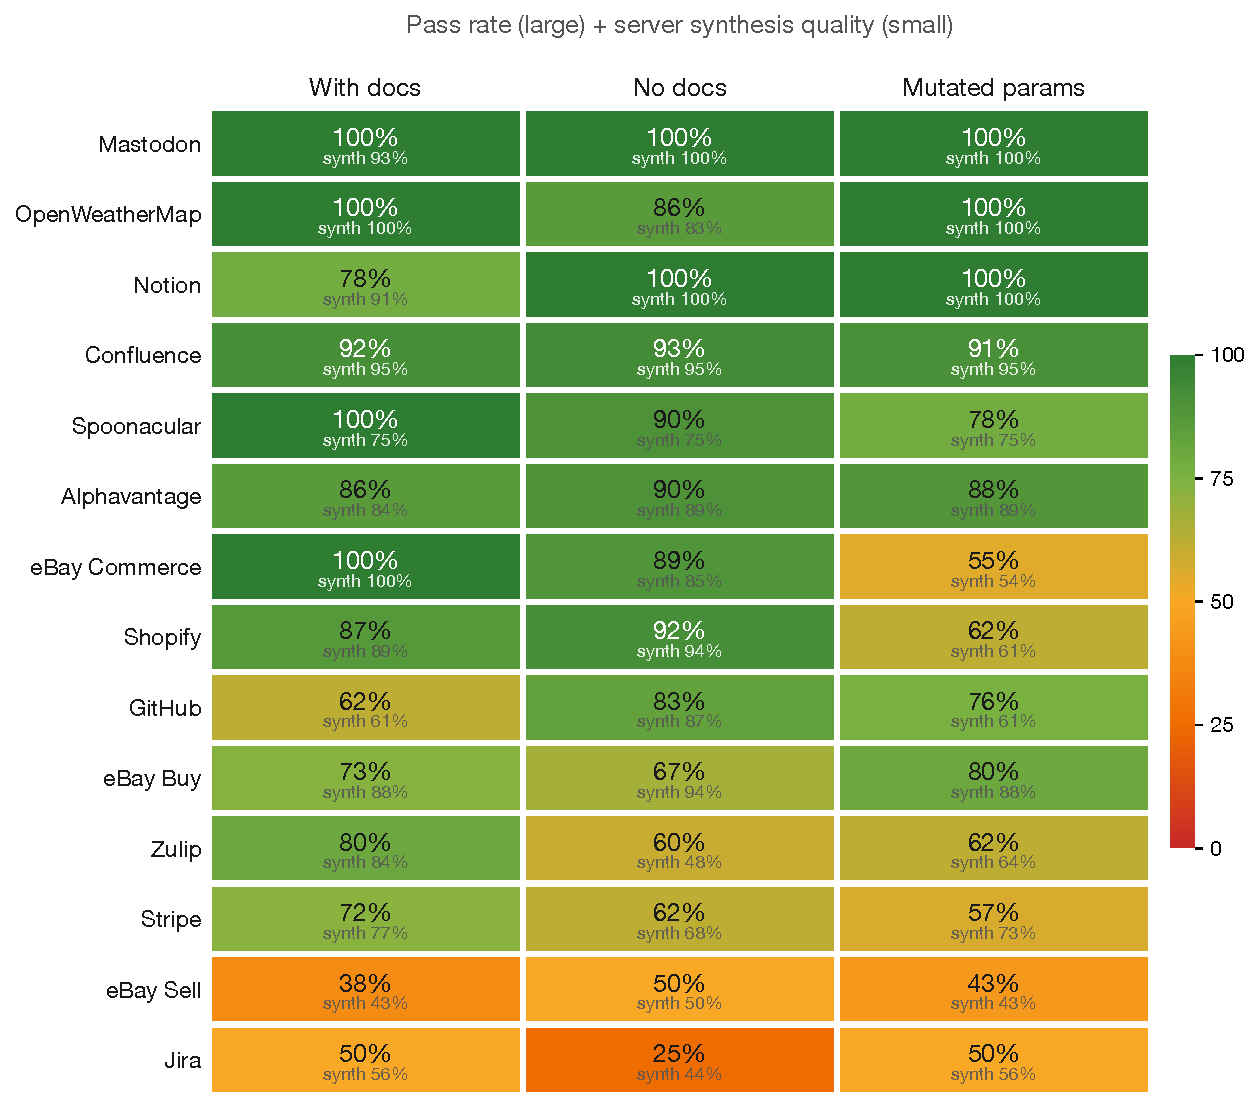
\includegraphics[width=\linewidth]{media/fig1_primary_heatmap.pdf}
  \caption{Agent pass rate (PASS, large) and server synthesis sufficiency
    (SYNTH, small) across 14 APIs and three synthesis conditions.
    Rows sorted by mean PASS descending.
    Colour encodes PASS on a red--orange--green scale.}
  \label{fig:heatmap}
\end{figure}

% ------------------------------------------------------------
\section{RQ2: Agent Task Completion}
\label{sec:rq2}
% ------------------------------------------------------------

\textbf{Do synthesized servers enable effective agent task completion, compared to human-authored references?}

Figure~\ref{fig:strip} shows the distribution of PASS across APIs and conditions. The median PASS is approximately 80\% in the docs condition and 86\% in the no-docs condition, with a long tail of high performers (Mastodon 100\% across all three conditions; Confluence 91--93\%; OpenWeatherMap 86--100\%) and a small floor group (Jira mean 42\%; eBay Sell mean 45\%).

The variance across APIs is explained by two distinct mechanisms. For the floor group, SYNTH is also low: Jira SYNTH=44--56\%, eBay Sell SYNTH=43\%. These are synthesis failures masquerading as agent failures --- when the required tools are absent, the agent cannot compensate. For APIs with moderate PASS but higher SYNTH (Stripe: SYNTH=77\%, PASS=72\%), the bottleneck shifts to agent reasoning on complex multi-step tasks. Figure~\ref{fig:scatter} makes this distinction visible: points near the diagonal are synthesis-limited; points below it are agent-limited.

\begin{figure}[htbp]
  \centering
  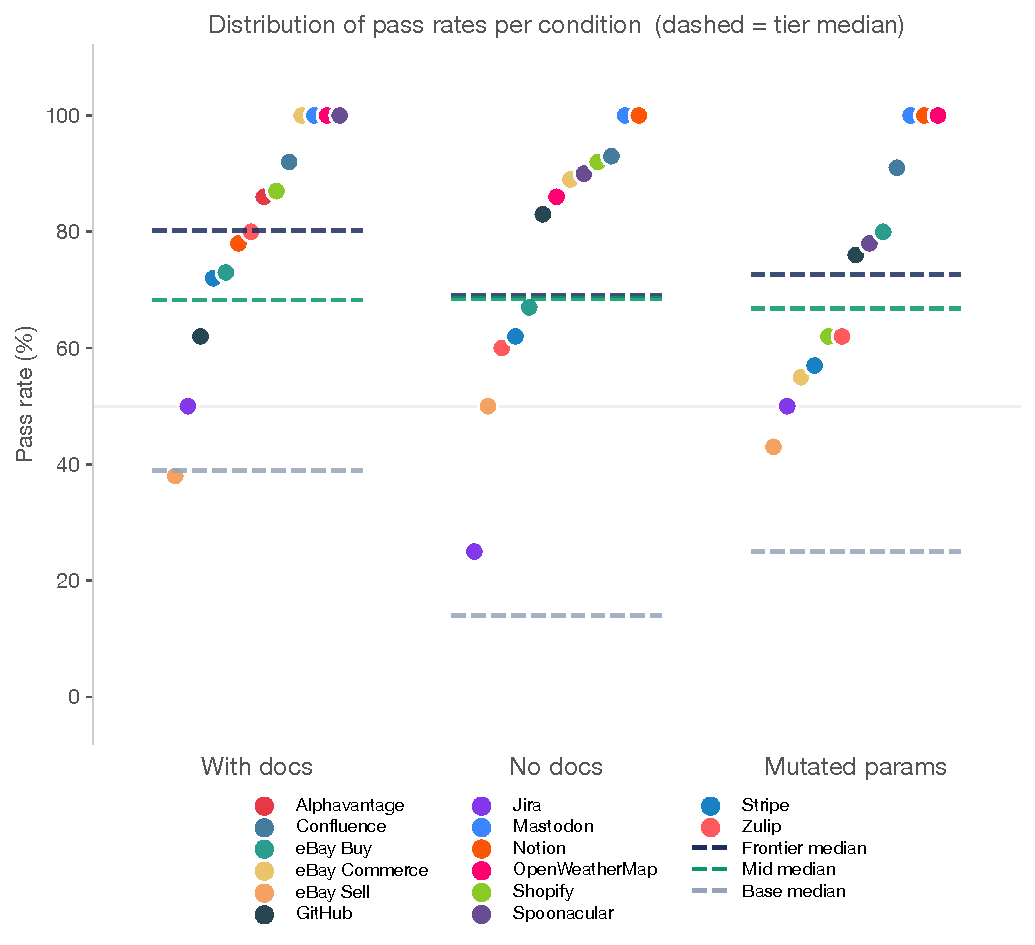
\includegraphics[width=0.85\linewidth]{media/fig2_condition_slopes.pdf}
  \caption{Distribution of PASS per synthesis condition.
    Each dot is one API; dashed line shows the median.
    The 50\% reference line is shown in light grey.}
  \label{fig:strip}
\end{figure}

\paragraph{Comparison with human-authored references.}
On GitHub, the community MCP server scores 65\% PASS. Synthesized servers with docs match this (62--67\% across valid runs), and synthesized servers without docs comfortably exceed it (83--90\%), because the synthesis model's parametric knowledge of the GitHub API produces more complete tool coverage than the hand-written reference. On Zulip, the community reference scores 68\%; the synthesized docs-condition server scores 80\%. In both cases the human reference fails on the same \texttt{TOOL\_COVERAGE} pattern --- missing webhooks, branch protection, and Actions dispatch for GitHub; message edit, DM search, and scheduled messages for Zulip ---while the synthesized server adds these endpoints.

% ------------------------------------------------------------
\section{RQ3: Parametric Knowledge and Documentation Faithfulness}
\label{sec:rq3}
% ------------------------------------------------------------

\textbf{To what extent do synthesizers rely on parametric knowledge rather than documentation, and does this affect performance?}

The mutated-docs condition directly operationalises this question: if a synthesizer adopts the renamed parameter names, it is reading the documentation; if it does not, it is writing from memory. Figure~\ref{fig:adherence} shows the PASS delta (mutated $-$ docs) per API alongside the interface-layer adherence rate (diamond markers). GitHub, Stripe, Shopify, Zulip, and Jira show near-zero adherence --- the synthesizer ignores mutations entirely and writes from training-time knowledge. Mastodon and Alphavantage reach full adherence, indicating the model follows provided documentation faithfully for less-familiar APIs.

The bar lengths directly test whether low adherence implies immunity to mutation. GitHub fits: near-zero adherence, bar near zero ($-$14 pp, offset by nodocs improvements visible in Fig.~\ref{fig:docs_effect}). Stripe does not: also near-zero adherence, yet mutation still costs 15 pp. This confirms that parametric reliance at synthesis does not cleanly propagate to agent performance.

The mechanism behind this is that the effect of parametric reliance depends on whether the synthesis model and the evaluation agent share the same prior. When both ignore mutations and operate from training-time knowledge --- as for GitHub --- the mutation is invisible to the whole pipeline and performance is unaffected. When the synthesizer adopts mutations faithfully (high adherence) but the evaluation agent's prior does not anticipate the renamed parameters, performance degrades. The contamination is only detectable as a problem when the two components have mismatched priors.

\begin{figure}[htbp]
  \centering
  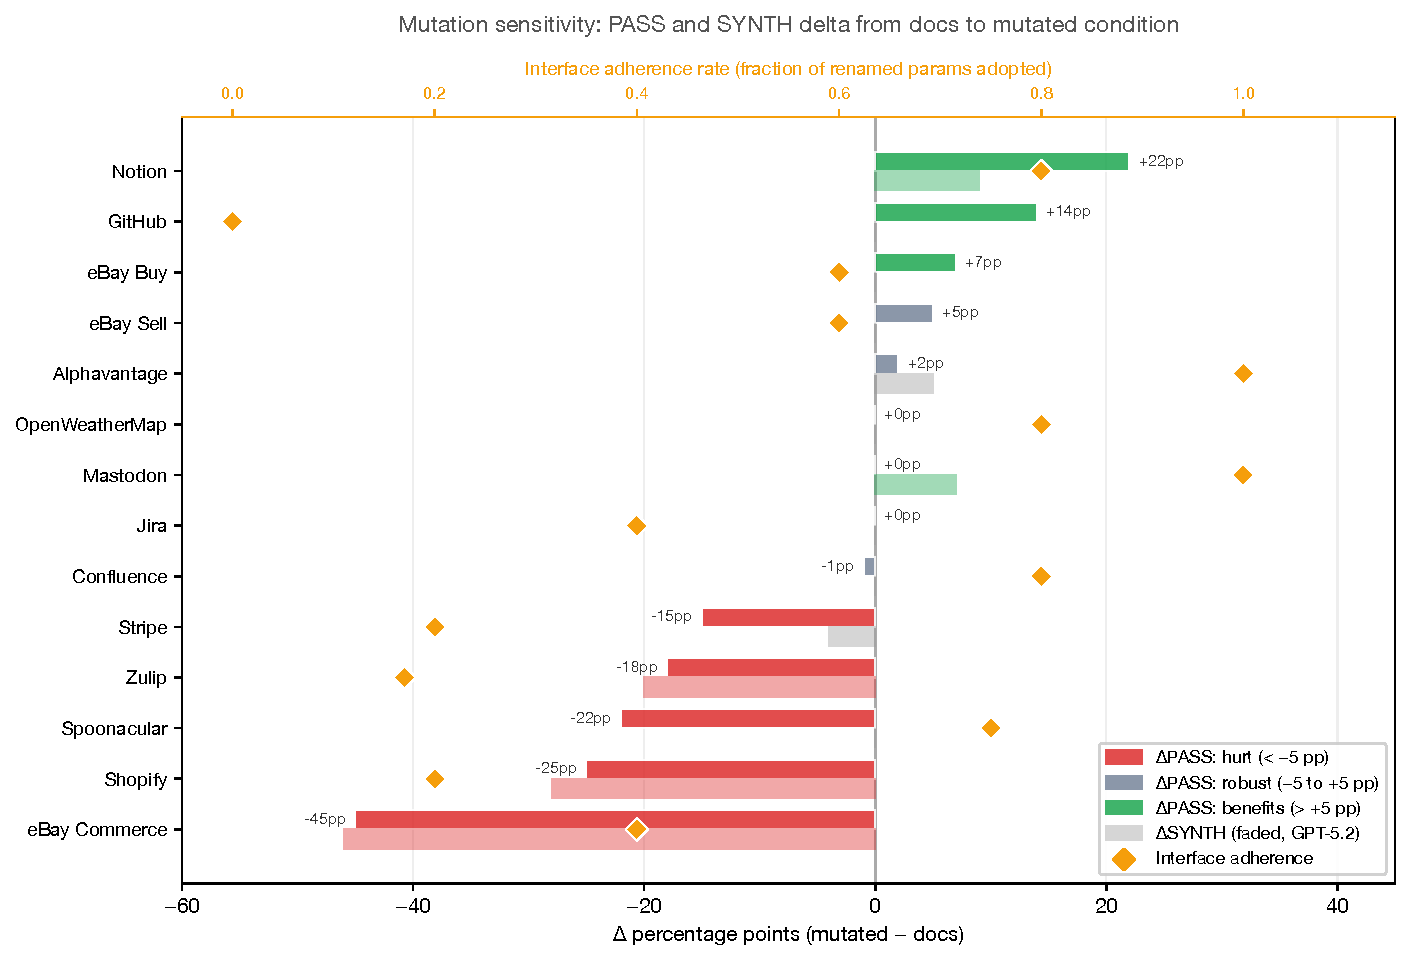
\includegraphics[width=\linewidth]{media/fig6_mutation_sensitivity.pdf}
  \caption{PASS delta (mutated $-$ docs, in percentage points) per API, sorted
    ascending. Red bars indicate APIs hurt by parameter renaming; green bars
    indicate APIs that benefit or are unaffected. Diamond markers (amber) show
    the interface-layer mutation adherence rate: how many renamed parameters the
    synthesizer adopted. Low adherence implies the synthesizer relied on
    parametric knowledge rather than the provided documentation.}
  \label{fig:adherence}
\end{figure}

% ------------------------------------------------------------
\section{RQ4: Effect of Documentation Availability}
\label{sec:rq4}
% ------------------------------------------------------------

\textbf{How does documentation availability affect synthesis and agent
performance?}

Figure~\ref{fig:strip} shows the median PASS per condition. The no-docs median (86\%) meets or exceeds the docs median (80\%), indicating that removing documentation does not on average degrade agent performance. This aggregate result conceals meaningful per-API variation, visible in Figure~\ref{fig:docs_effect}.

\begin{figure}[htbp]
  \centering
  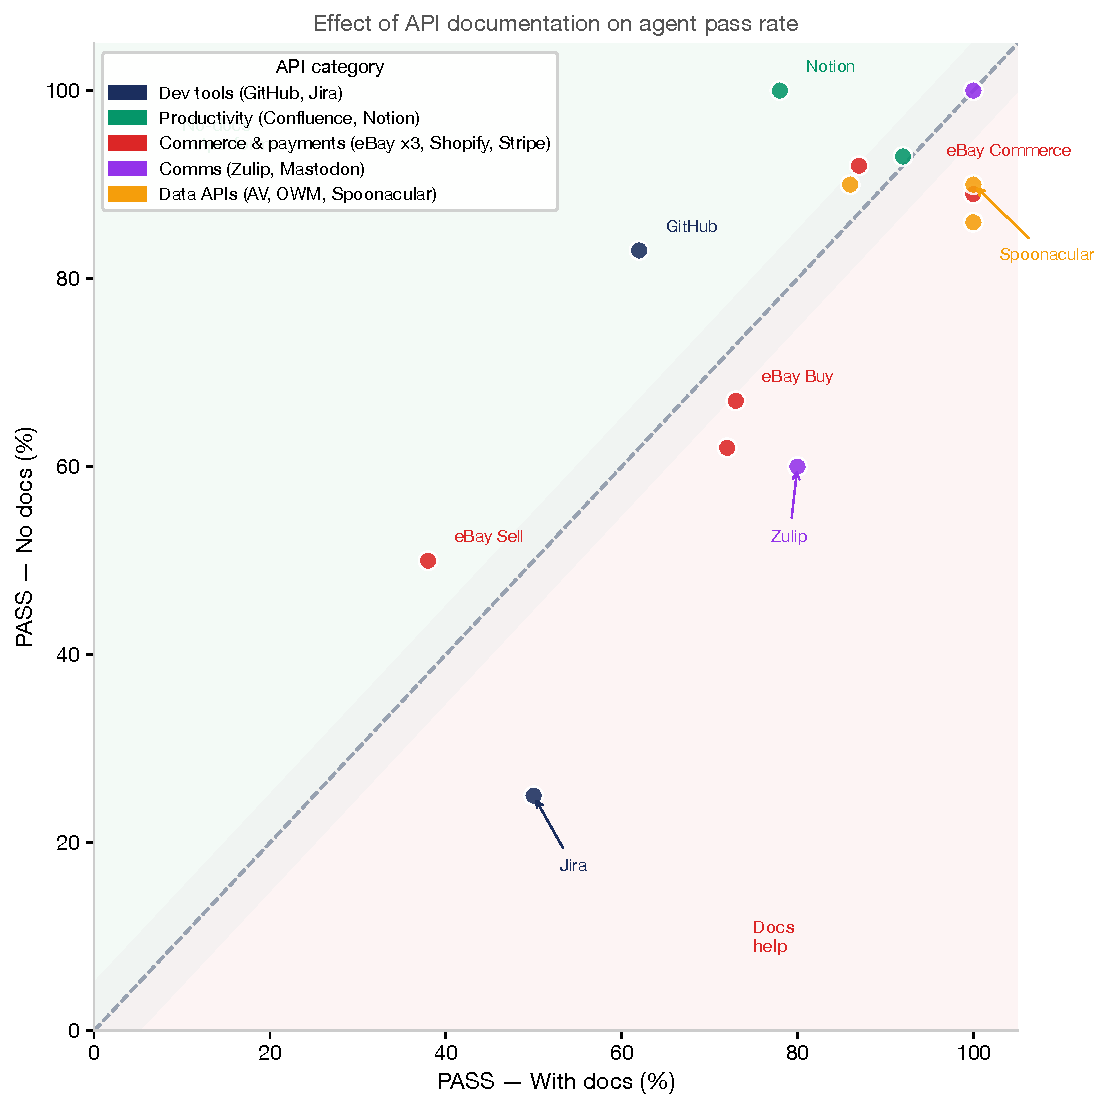
\includegraphics[width=0.72\linewidth]{media/fig7_docs_effect.pdf}
  \caption{Docs vs.\ no-docs PASS per API. Points above the diagonal
    indicate APIs where removing documentation improved performance;
    points below indicate APIs where documentation helped.}
  \label{fig:docs_effect}
\end{figure}

APIs above the diagonal (nodocs wins) include GitHub, Notion, and Mastodon: high-frequency, well-documented APIs for which the synthesis model has strong training-time priors. Removing documentation reduces noise and allows the model to produce a clean, complete server from memory. APIs below the diagonal (docs help) include Stripe and Zulip: less saturated in training
data, or with API conventions sufficiently idiosyncratic that documentation provides genuine signal the model could not otherwise recover.

The mutated condition (also visible in Figure~\ref{fig:strip}) shows a modest further decrease in the median (77\%), indicating that parameter renaming does introduce some degradation on average. However, the APIs most sensitive to mutation are precisely those with high adherence (Section~\ref{sec:rq3}), consistent with the interpretation that harm from mutations is mediated by whether the synthesizer adopted them.

% ------------------------------------------------------------
\section{RQ5: Synthesis Quality as a Predictor of Agent Performance}
\label{sec:rq5}
% ------------------------------------------------------------

\textbf{Does synthesis quality predict agent task performance?}

Figure~\ref{fig:scatter} plots SYNTH against PASS for all 42 API--condition pairs. The Pearson correlation is $r = 0.895$ ($p < 0.0001$, $n = 42$), indicating a strong linear relationship between synthesis sufficiency and agent pass rate. This is the central methodological validation result: SYNTH is a reliable proxy for downstream utility, and failures in synthesis propagate to agent failures with high fidelity.

\begin{figure}[htbp]
  \centering
  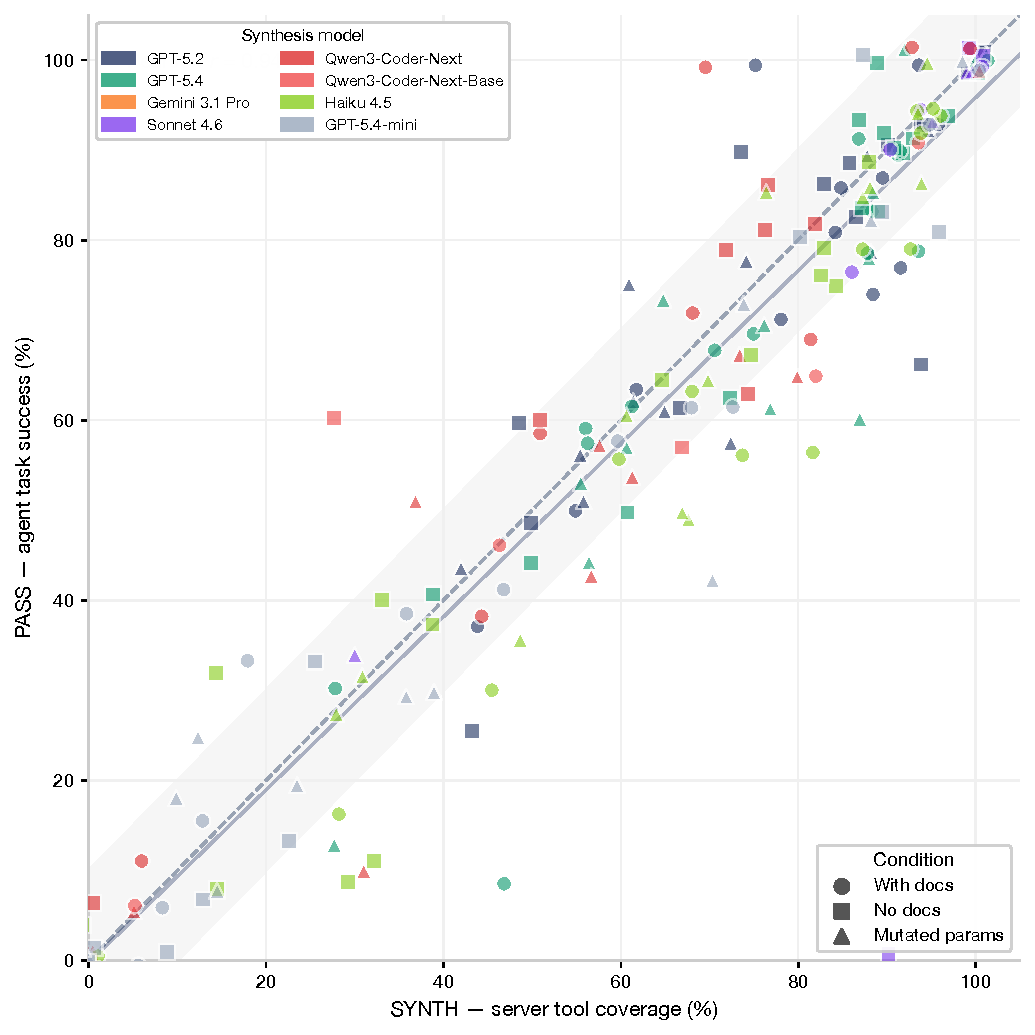
\includegraphics[width=0.72\linewidth]{media/fig4_synth_scatter.pdf}
  \caption{SYNTH vs.\ PASS across all 42 API--condition pairs
    ($r = 0.895$). Shape encodes synthesis condition;
    colour encodes API category.
    The dashed line is $y = x$; the grey band is $\pm 10$ pp.}
  \label{fig:scatter}
\end{figure}

The points near or above the diagonal represent cases where the agent performs at or above what synthesis quality would predict --- most commonly when the agent compensates for minor coverage gaps with general reasoning (Spoonacular: SYNTH=75\%, PASS=100\% in the docs condition). Points well below the diagonal (eBay Commerce mutated: SYNTH=54\%, PASS=55\%) confirm that when synthesis fails to cover the task space, agent performance cannot recover. The Jira no-docs outlier (SYNTH=44\%, PASS=25\%) represents the most severe case of synthesis-induced failure in the benchmark.

Taken together, these results validate SYNTH as a leading indicator: measuring synthesis sufficiency before running the full evaluation pipeline gives a reliable estimate of whether agent task completion will succeed.

% ------------------------------------------------------------
\section{Model Comparison}
\label{sec:model_comparison}
% ------------------------------------------------------------

\textbf{How does synthesis model capability affect agent pass rate?}

To isolate model effects from API-specific variation, we evaluate eight synthesis models on a common three-API set (GitHub, Stripe, Zulip) selected to span low, medium, and high familiarity. Table~\ref{tab:model_comparison} reports PASS for all models across all three APIs and conditions; absent conditions are synthesis failures (no runnable server produced) and score as 0\%. Figure~\ref{fig:model_capability} summarises the per-model distributions. Qwen3-Coder-Next-Base has very sparse coverage on this set --- GitHub produced no valid server in any condition, and only single conditions were evaluated for Stripe and Zulip --- reflecting the limits of a base model without instruction tuning.

Sonnet~4.6 achieves the highest median PASS across the three APIs. GPT-5.2, GPT-5.4, and Haiku~4.5 form a competitive mid-tier, though with distinct failure modes: GPT-5.4 produces broken tool stubs for Stripe docs (8\%) --- a synthesis-level failure confirmed by SYNTH=48\% --- while Haiku~4.5 collapses on Zulip nodocs (36\%) and mutated (26\%), indicating weaker parametric coverage of that API. Gemini~3.1 Pro is broadly competitive at mid-tier for GitHub and Zulip but weaker on Stripe.

The two weakest models show qualitatively different failure patterns. GPT-5.4-mini consistently produces shallow servers with too few relevant tools (TOOL\_COVERAGE dominates across all nine conditions, −43\,pp below GPT-5.2 on average). Qwen3-Coder-Next has high crash rates --- Stripe docs and mutated, and Zulip docs and nodocs all produce servers that fail on startup --- but achieves competitive results on the conditions where synthesis succeeds (GitHub: 57--60\%, Zulip mutated: 64\%, Stripe nodocs: 62\%).

Synthesis reliability --- the fraction of conditions producing a runnable server --- scales with model tier. Sonnet~4.6, GPT-5.2, and Gemini~3.1 Pro achieve near-complete reliability across all nine conditions. Qwen3-Coder-Next fails on four of nine; GPT-5.4-mini produces a server for all nine but with coverage too thin to be useful (SYNTH 14--48\%).

The nodocs advantage observed in RQ4 is strongest for larger models. Sonnet~4.6 and GPT-5.2 improve or hold steady on GitHub when documentation is removed, consistent with strong parametric priors overriding documentation noise. Qwen3-Coder-Next, by contrast, shows 60\% interface-layer adherence on GitHub and Stripe (though 0\% HTTP adherence --- the renamed parameters are reflected in Python signatures but not in outbound API calls), indicating it reads documentation more literally but does not fully propagate renames to execution.

This model-level variation in adherence is a confound when interpreting the aggregate adherence results in Section~\ref{sec:rq3}: the near-zero aggregate adherence for GitHub reflects a mixture of high-capability models ignoring mutations entirely (parametric dominance) and lower-capability models adopting renames at the interface level but not the HTTP level. The full per-model adherence breakdown is reported in Appendix~\ref{sec:apx:full_results}.

\begin{table}[htbp]
  \centering
  \caption{PASS (\%) on the common three-API set by synthesis model and condition.
    Models ordered by approximate capability (ascending left to right).
    0\% cells marked \colorbox{red!12}{red} include both true zeros and synthesis crashes.
    Shaded rows are the two weakest models.}
  \label{tab:model_comparison}
  \setlength{\tabcolsep}{3.5pt}
  \scriptsize
  \begin{tabular}{ll rrr rrr rrr}
    \toprule
    & & \multicolumn{3}{c}{\textbf{GitHub}} & \multicolumn{3}{c}{\textbf{Stripe}} & \multicolumn{3}{c}{\textbf{Zulip}} \\
    \cmidrule(lr){3-5}\cmidrule(lr){6-8}\cmidrule(lr){9-11}
    \textbf{Model} & & D & N & M & D & N & M & D & N & M \\
    \midrule
    \rowcolor{gray!10}
    GPT-5.4-mini          & & 38 & 32 & 30 & 14 & \cellcolor{red!12}0 & 19 & 40 & 14 & 29 \\
    \rowcolor{gray!10}
    Qwen3-Coder-Next-Base & & \cellcolor{red!12}0 & \cellcolor{red!12}0 & \cellcolor{red!12}0 & \cellcolor{red!12}0 & 56 & \cellcolor{red!12}0 & \cellcolor{red!12}0 & \cellcolor{red!12}0 & \cellcolor{red!12}0 \\
    \rowcolor{gray!10}
    Qwen3-Coder-Next      & & 58 & 60 & 57 & \cellcolor{red!12}0 & 62 & \cellcolor{red!12}0 & \cellcolor{red!12}0 & \cellcolor{red!12}0 & 64 \\
    Gemini~3.1 Pro        & & \textbf{78} & 71 & 36 & 47 & 50 & 59 & 76 & \textbf{84} & 62 \\
    GPT-5.2               & & 62 & 83 & 76 & \textbf{72} & 62 & 57 & \textbf{80} & 60 & 62 \\
    GPT-5.4               & & 58 & \textbf{89} & 73 & 8 & 62 & 12 & \textbf{90} & 85 & 71 \\
    Haiku~4.5             & & \textbf{95} & 90 & \textbf{86} & 57 & \textbf{75} & \textbf{86} & 55 & 36 & 26 \\
    Sonnet~4.6            & & 90 & \textbf{100} & \textbf{100} & 77 & \textbf{100} & \textbf{100} & \textbf{100} & 43 & \cellcolor{red!12}0 \\
    \bottomrule
  \end{tabular}
  \par\smallskip
  \raggedright\scriptsize D = docs, N = nodocs, M = mutated.
  Bold = highest per column. Shaded rows = weakest models.
  Qwen3-Coder-Next-Base GitHub: no server.py produced; Stripe/Zulip: only one condition evaluated.
  Sonnet~4.6 Zulip mutated: synthesis stream error on all attempts.
\end{table}

\begin{figure}[htbp]
  \centering
  
\includegraphics[width=\linewidth]{media/fig9_model_capability.pdf}
  \caption{PASS distributions for seven synthesis models on the common
    three-API set (GitHub, Stripe, Zulip), ordered by approximate capability.
    Each box shows nine data points (3 APIs $\times$ 3 conditions);
    crash/failure conditions count as 0\%.}
  \label{fig:model_capability}
\end{figure}

\begin{figure*}[htbp]
  \centering
  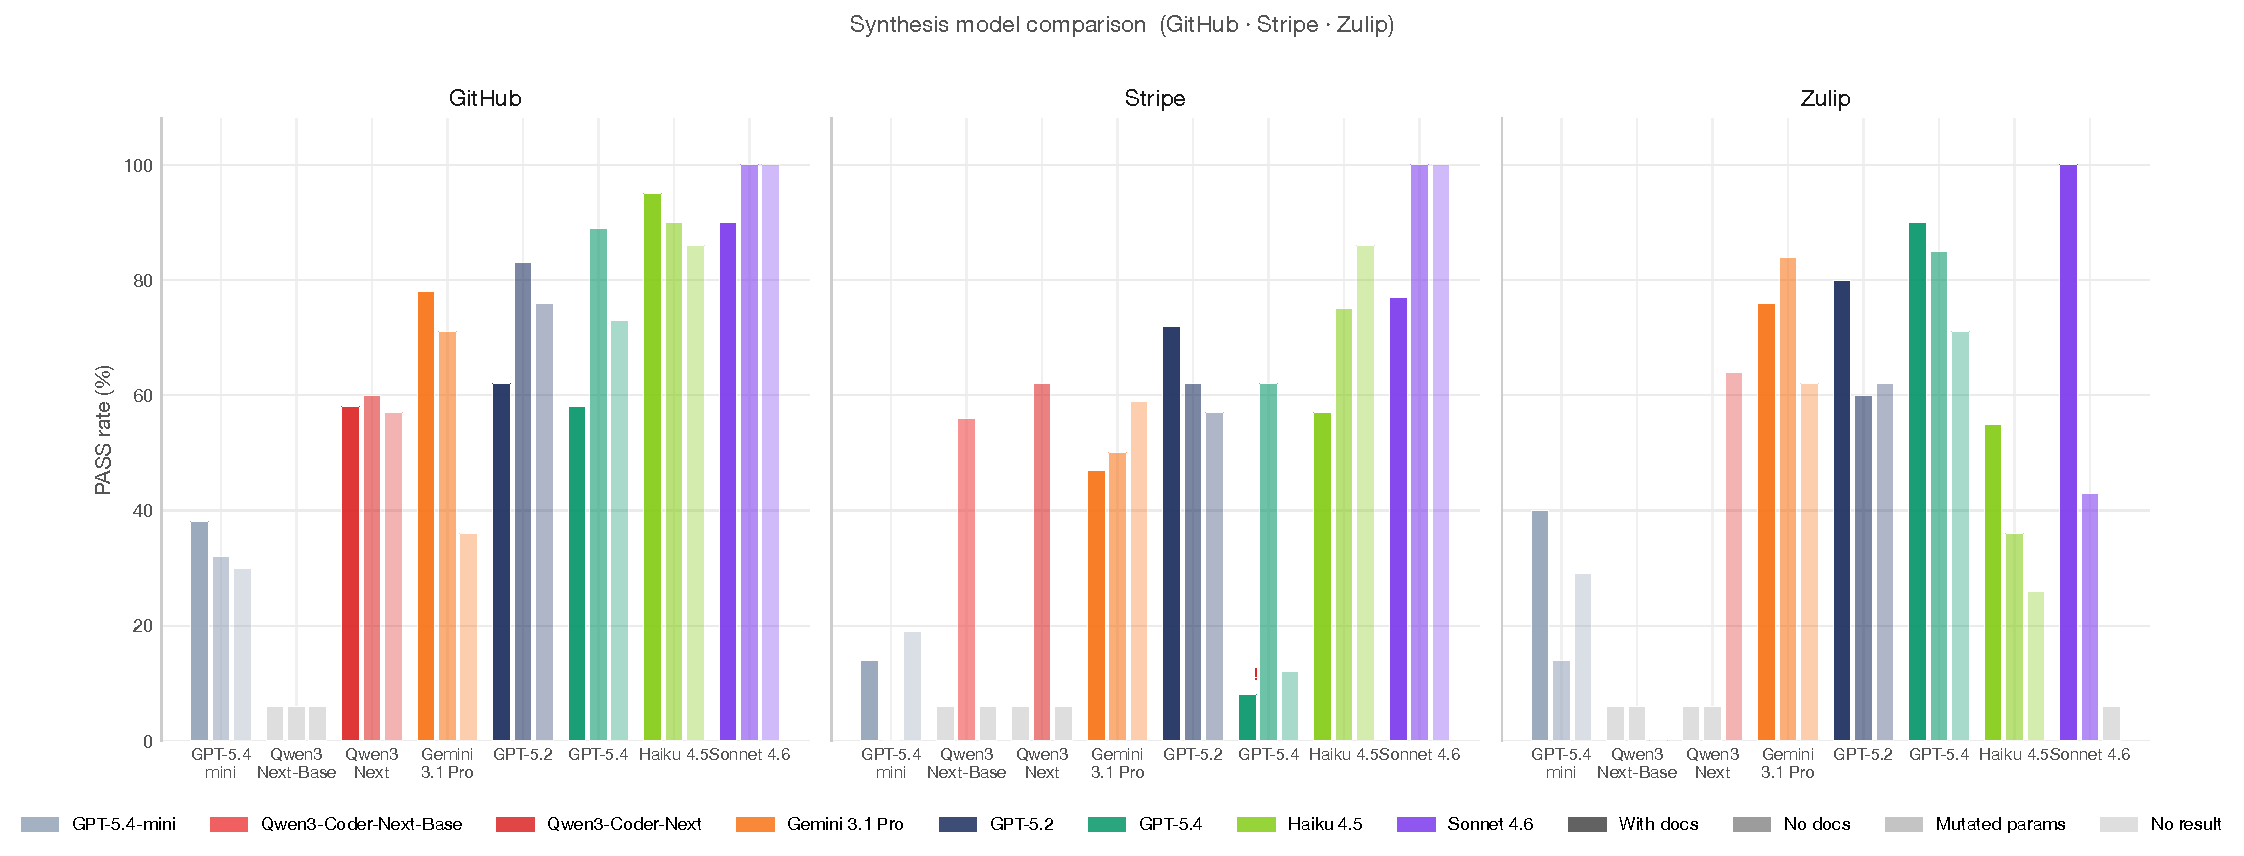
\includegraphics[width=\linewidth]{media/fig3_model_comparison.pdf}
  \caption{Per-API, per-model PASS breakdown across all synthesis conditions
    (docs, nodocs, mutated) for the common three-API set. Each group of bars
    corresponds to one API; colours distinguish synthesis models.
    Zero-height bars indicate synthesis crashes or complete tool-coverage failure.
    The GPT-5.4 Stripe docs bar (8\%) reflects broken tool stubs, not agent failure.}
  \label{fig:model_comparison}
\end{figure*}
